\documentclass[letterpaper]{article}
\usepackage[submission]{aaai2027}
\usepackage[hyphens]{url}
\usepackage{graphicx}
\graphicspath{{./}{../}}
\urlstyle{rm}
\def\UrlFont{\rm}
\usepackage{natbib}
\usepackage{caption}
\frenchspacing

\usepackage{amsmath}
\usepackage{amssymb}
\usepackage{booktabs}
\usepackage{array}

\ifdefined\pdfinfo
\pdfinfo{
/TemplateVersion (2027.1)
}
\fi

\setcounter{secnumdepth}{2}

\newcommand{\ours}[1]{\textbf{#1 (Ours)}}
\newcommand{\oursnum}[1]{\(\boldsymbol{#1}\)}
\newcommand{\ourscell}[1]{\textbf{#1}}

\title{\title{SABER: Support-Conditioned Bellman Error Reweighting\\
for Sparse-Reward Hindsight Experience Replay}}
\author{Anonymous Submission}
\affiliations{}

\begin{document}
\maketitle

\begin{abstract}
Hindsight Experience Replay (HER) converts failed trajectories into goal-conditioned training data through achieved-goal relabeling. While prior extensions mainly modify goal selection, replay sampling, or target construction, we study how critic losses should be allocated after relabeling and sampling are fixed. We introduce SABER, a critic-only objective that adaptively reweights squared Bellman residuals using local replay support. A transition receives greater weight when its state-goal-horizon neighborhood is sufficiently populated and contains actions consistent with the current policy. The current-policy action is used only for the support query, while Bellman regression remains defined at the replay action. SABER leaves HER relabeling, uniform replay, actor updates, Bellman targets, network architectures, and the update-to-data ratio unchanged. Under matched UTD-1 training on FetchPickAndPlace, SABER improves normalized success AUC by 0.070 to 0.112 across DDPG, TD3, and SAC. On DrawerOpen with DDPG, it raises mean AUC from 0.207 to 0.754 and mean final success from 0.390 to 1.000. Controlled comparisons, ablations, and diagnostics distinguish SABER from alternative loss-allocation mechanisms and characterize its support signal. These results establish post-HER critic-loss reweighting as a distinct design axis that can substantially improve performance without changing the surrounding HER pipeline or increasing the update budget.
\end{abstract}

\section{Introduction}


\begin{figure}[!htb]
\centering
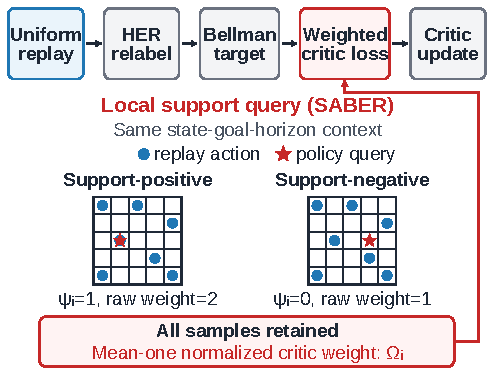
\includegraphics[width=\columnwidth]{figures/saber_pipeline_weighting.pdf}
\caption{SABER reweights post-HER critic residuals using same-context replay support for the current-policy action; all samples are retained.}
\label{fig:saber-method-overview-submission}
\end{figure}

A central challenge in sparse-reward goal-conditioned reinforcement learning is obtaining useful supervision when successful trajectories are rare. Hindsight Experience Replay (HER) addresses this challenge by relabeling failed experience with achieved goals~\citep{andrychowicz2017her}. Once sampling and relabeling are fixed, however, standard HER actor--critics assign equal coefficients to all sampled Bellman residuals. This uniform objective ignores a structural mismatch in off-policy actor--critic learning: the critic is fitted at historical replay actions, whereas the actor is updated using critic values at actions proposed by the current policy.

The relevance of a sampled residual to the actor update may therefore depend on the replay evidence available near the action that the actor currently proposes. Consider two relabeled samples with comparable Bellman errors. In one state--goal--horizon context, replay contains actions in the same local action region as the current-policy action; in the other, it does not. Treating the two residuals identically discards this observable difference in local support. This does not imply that unsupported samples should be removed, nor that support estimates value accuracy or uncertainty. It instead motivates a narrower allocation principle: retain every sampled transition and Bellman target, but devote relatively more critic fitting to samples whose local replay context contains evidence near the action at which the actor queries the critic.

We introduce SABER (Support-Conditioned Adaptive Bellman Error Reweighting), a critic-only post-HER objective. SABER tests whether replay actions from the same discretized state--goal--horizon context occupy the current-policy action bin, upweights support-positive residuals, and normalizes weights to unit minibatch mean. The current-policy action is used only for this support query; regression remains at the replay action. Relabeling, replay sampling, rewards, Bellman targets, actor optimization, architectures, and the update budget remain unchanged. Unlike replay prioritization, which changes which transitions enter the minibatch, SABER preserves minibatch membership and changes only coefficients of critic residuals after sampling and relabeling.

Across seven matched task--backbone cohorts, SABER improves mean normalized success AUC over standard HER in every cohort, with paired confidence intervals excluding zero in four. The improvement is repeatable across DDPG, TD3, and SAC on FetchPickAndPlace and is particularly large on DrawerOpen with DDPG, where mean AUC rises from 0.207 to 0.754. Diagnostic analyses show that support-positive samples are enriched, but not reducible to, high-TD-error samples and undergo consistently larger residual reductions after one critic update. At the same time, comparisons with HGR and PER reveal task- and backbone-dependent orderings, positioning SABER as a distinct loss-allocation mechanism rather than a universally dominant replacement for replay prioritization.

Our contributions are threefold:
\begin{itemize}
    \item We formulate post-HER critic-loss allocation as a design axis distinct from goal selection, replay prioritization, and target construction.

    \item We introduce SABER, a critic-only objective that reweights Bellman residuals using local support for the current-policy action without changing the surrounding HER pipeline.

    \item We evaluate SABER across DDPG, TD3, and SAC using matched baselines, controlled variants, and mechanism diagnostics, and characterize both its gains and task-dependent limitations.
\end{itemize}

\section{Related Work}

Universal value function approximators formalize generalization across goals~\citep{schaul2015uvfa}, while recent theory characterizes sample-efficiency gains from goal relabeling~\citep{zheng2024goalrelabeling}. Around HER, methods modify several stages. Hindsight Goal Generation (HGG) generates goals that balance short-term reachability with progress toward the desired goal~\citep{ren2019hgg}. Curriculum-guided Hindsight Experience Replay (CHER) selects hindsight experiences through a curriculum based on goal proximity and pseudo-goal diversity~\citep{fang2019cher}. Energy-Based Prioritization (EBP) prioritizes episodes by object-trajectory energy~\citep{zhao2018ebp}. Hindsight Goal Ranking (HGR) instead prioritizes both episodes and transition--future-goal pairs by temporal-difference (TD) error with two-stage importance correction~\citep{luu2021hgr}. Multi-step Hindsight Experience Replay (MHER) uses multi-step relabeled returns~\citep{yang2023mher}, Aggressive Rewards to Counter Bias in Hindsight Experience Replay (ARCHER) rescales hindsight rewards~\citep{lanka2018archer}, and Unbiased Sampling for Hindsight Experience Replay (USHER) corrects hindsight-induced value bias in stochastic environments~\citep{schramm2023usher}.

General replay methods redistribute experience independently of HER. Prioritized Experience Replay (PER) samples by TD error with importance correction~\citep{schaul2016per}. Under suitable transformations, non-uniform sampling and a uniformly sampled loss can induce the same expected gradient~\citep{fujimoto2020equivalence}. Regret Minimization Experience Replay further derives priorities from Bellman error, on-policiness, and value accuracy~\citep{liu2021regret}. Attentive Experience Replay (AER) selects transitions according to state similarity with the agent's current state~\citep{sun2020aer}. Remember and Forget for Experience Replay (ReF-ER) suppresses far-policy samples while regularizing the actor toward replay behavior~\citep{novati2019refer}.

Action support is also central in offline RL: BCQ restricts policy actions toward the batch distribution, BEAR constrains backup actions through support matching, and CQL conservatively regularizes values on out-of-distribution actions~\citep{fujimoto2019bcq,kumar2019bear,kumar2020cql}. SABER instead trains online with HER, constrains neither the actor nor Bellman target, and uses local support only to allocate coefficients among replay-action residuals.

Closer critic-reweighting methods learn different signals. Experience Replay with Likelihood-Free Importance Weights estimates a current-policy-to-replay density ratio~\citep{sinha2022lfiw}. Distribution Correction (DisCor) reweights samples according to estimated target accuracy~\citep{kumar2020discor}. ReenGAGE adds gradient-based knowledge distillation to goal-conditioned critic learning~\citep{levine2023reengage}. Across these lines, SABER differs in its implemented intervention and support signal. After HER relabeling and replay sampling are fixed, it preserves minibatch membership, rewards, targets, and the actor objective, and uses a non-learned, sample-aligned current-policy action-support predicate only to set critic-loss coefficients. It uses no density ratio, target-error model, or auxiliary target.

\section{SABER}\label{sec:saber}

\subsection{Problem Formulation and the Post-HER Critic-Loss Allocation Gap}

We consider a finite-horizon goal-conditioned Markov decision process
\(\mathcal M=(\mathcal S,\mathcal A,\mathcal G,P,r,\gamma,H)\).
At time \(t\), the environment is in state \(s_t\in\mathcal S\), the
agent receives observation \(o_t=\omega(s_t)\), and the desired goal is
\(g\in\mathcal G\).  The goal-conditioned input is \(x_t=(o_t,g)\), and
the policy and critic are denoted by
\(\pi_\theta(a\mid x)\) and \(Q_{\phi_k}(x,a)\), respectively.  Let
\(m:\mathcal S\rightarrow\mathcal G\) map a state to its achieved goal.
The environment provides the sparse goal-conditioned reward
\begin{equation}
r(s_t,a_t,s_{t+1},g)=
\begin{cases}
0, & d\!\left(m(s_{t+1}),g\right)\leq\epsilon_g,\\
-1, & \text{otherwise}.
\end{cases}
\end{equation}
When successful trajectories are rare, replay collected under the
original desired goal contains little direct successful supervision.

Let an episode contain states \(s_0,\ldots,s_T\) and transitions
indexed by \(t=0,\ldots,T-1\). In our future-goal HER
implementation~\citep{andrychowicz2017her}, a transition selected for
relabeling samples a later stored transition \(u\) and uses its next
achieved goal:
\begin{equation}
\begin{aligned}
u &\sim \operatorname{Unif}\{t+1,\ldots,T-1\},\\
\tilde g_i &= m(s_{u+1}),\\
\tilde r_i &= r(s_t,a_t,s_{t+1},\tilde g_i).
\end{aligned}
\end{equation}
When the eligible set is empty, or when a transition is not selected
for relabeling, the original desired goal is retained. The resulting network inputs are
\(x_i=(o_i,\tilde g_i)\) and \(x_i'=(o_i',\tilde g_i)\).  For backbone
\(\mathsf A\), let \(y_i^{\mathsf A}\) denote its standard Bellman
target after relabeling and reward recomputation.  For critic \(k\),
the replay-action Bellman residual is
\begin{equation}
\delta_{ik}
=Q_{\phi_k}(x_i,a_i^r)-y_i^{\mathsf A},
\end{equation}
where \(a_i^r\) is the action stored in replay.  Given a uniformly
sampled and relabeled minibatch \(B\), the standard HER critic
objective is
\begin{equation}
\mathcal L_Q^{\mathrm{HER}}
=\frac{1}{|B|}
\sum_{i\in B}\sum_{k=1}^{n_Q}\delta_{ik}^{2}.
\end{equation}
Thus, once replay sampling and relabeling are fixed, every sampled
residual receives the same explicit coefficient.

HER determines which relabeled goals and rewards are used for
learning, but it does not determine how critic fitting effort should
be distributed among the residuals in the resulting minibatch.  This
gap may matter in off-policy actor--critic learning: the critic
regresses Bellman targets at replay actions \(a_i^r\), whereas the
actor improves the policy by querying the critic at current-policy
actions \(a_i^\pi\).  The amount of replay evidence near these policy
queries can vary across observation-derived state--goal contexts.  We therefore ask
whether observable local replay support for \(a_i^\pi\) can be used
to allocate critic-loss weight while holding the relabeled minibatch
and Bellman targets fixed.

Because this question requires both replay evidence and a replay-based
critic objective, SABER is designed for replay-based off-policy
actor--critic learning.  We instantiate it with three representative
continuous-control backbones: DDPG~\citep{lillicrap2016ddpg}, which uses a deterministic actor
and one critic; TD3~\citep{fujimoto2018td3}, which uses a deterministic actor, twin critics,
target-policy smoothing, and delayed actor updates; and SAC, which
uses a stochastic entropy-regularized actor and twin
critics~\citep{haarnoja2018sac}.
These algorithms provide representative deterministic and stochastic
off-policy structures while retaining the replay-based critic update
required by SABER.  SABER leaves each backbone's Bellman target,
bootstrap convention, and actor objective unchanged.

\subsection{SABER Overview and Intervention Point}

SABER is a per-sample critic-loss objective, not a network layer or
replay sampler. As Fig.~\ref{fig:saber-method-overview-submission}
shows, it acts after uniform replay, HER relabeling, reward
recomputation, and target construction but before critic-loss
reduction. For each relabeled sample, it queries whether the
current-policy action bin is occupied by same-context replay actions
and applies the resulting normalized weight to the Bellman residual
at the original replay action. All sampled transitions, relabeled
goals, rewards, and targets remain unchanged.

\subsection{Current-Policy Local Support}

For sample \(i\), SABER constructs a task-specific discrete
state--goal--horizon context from the agent-observed input, represented
by the full support-context key
\begin{equation}
c_i=C(o_i,\tilde g_i,h_i),
\end{equation}
where \(h_i\) is the remaining horizon. Here, ``state'' refers only to
task-relevant state features derived from \(o_i\), not to privileged
simulator state \(s_i\). In the manipulation domains
evaluated in Sec.~\ref{sec:experiments}, the full key summarizes task progression,
agent--object interaction, goal-relative geometry, gripper state, and
remaining horizon.  Concretely, FetchPickAndPlace uses manipulation
phase, hand--object distance, object--goal distance, object height,
gripper gap, and remaining horizon.  The Drawer tasks use interaction
phase, hand--handle distance, handle--goal distance, handle position
along the opening axis, gripper state, and remaining horizon.  These
features are discretized using fixed, task-specific bins.

To bound lookup cost, SABER first uses a lower-dimensional
\emph{coarse retrieval key} \(C^{\mathrm{ret}}(o,h)\), constructed
from a subset of the full-key components, only to retrieve candidate
replay slots. Let \(\mathbf J_i^{\mathrm{ret}}\) denote the ordered
list of currently valid, unique slots returned by the maintained index
for the query's coarse retrieval key. Invalid entries and duplicate
slot identifiers are removed in index order, retaining the first valid
occurrence. SABER examines at most \(N_{\mathrm{scan}}\) candidates:
\begin{equation}
S_i=
\operatorname{Tail}_{N_{\mathrm{scan}}}
\left(\mathbf J_i^{\mathrm{ret}}\right),
\qquad |S_i|\leq N_{\mathrm{scan}}.
\end{equation}
Here the tail is taken in the index's deterministic maintained order
and is not interpreted as temporal recency.
The coarse retrieval key is an indexing device, not the support
criterion.  Candidates are filtered using the full support-context
key:
\begin{equation}
I_i=
\left\{
j\in S_i:
C(o_j,\tilde g_i,h_j)
=C(o_i,\tilde g_i,h_i)
\right\}.
\end{equation}
This equality is exact component-wise matching: a candidate is
retained only when every discretized component of its full key equals
the corresponding query component.  The relabeled query goal
\(\tilde g_i\) is used to compute both sides of this comparison, so a
candidate is not matched using its originally stored desired goal.

Each action dimension is normalized by its environment bounds and
divided into \(K\) bins.  Let \(b_K(a)\) denote the resulting
multidimensional action bin and
\begin{equation}
\mathcal U_i=
\left\{
b_K(a_j^r)\mid j\in I_i
\right\}
\end{equation}
the set of replay-action bins occupied in the local context.  With
\(n_i=|I_i|\), SABER defines the support indicator
\begin{equation}
\psi_i=
\mathbf 1\!\left\{n_i\geq N_{\mathrm{local}}\right\}
\mathbf 1\!\left\{b_K(a_i^\pi)\in\mathcal U_i\right\}.
\end{equation}
The first condition requires a sufficiently populated local context;
the second tests whether the current-policy action bin has
been observed in that context.  The main setting uses
\begin{equation}
K=5,\qquad N_{\mathrm{scan}}=512,\qquad
N_{\mathrm{local}}=4.
\end{equation}
DDPG and TD3 use their deterministic actor action as \(a_i^\pi\).
For the support query, SAC uses the deterministic squashed mean of its
actor while retaining stochastic actions in its standard actor and
target objectives.  The indicator uses neither Q-values nor TD
errors.  It is a binary occupancy test, and the current-policy action
is not substituted for \(a_i^r\) in the Bellman residual.

\subsection{Normalized Critic-Only Objective and Backbone Integration}

SABER assigns the raw per-sample weight
\begin{equation}
w_i^{\mathrm{raw}}=1+\lambda_S\psi_i
\end{equation}
and normalizes the weights by their minibatch mean:
\begin{equation}
\bar w_B=
\frac{1}{|B|}\sum_{j\in B}w_j^{\mathrm{raw}},
\qquad
\Omega_i=
\frac{w_i^{\mathrm{raw}}}
{\max(\epsilon_w,\bar w_B)}.
\end{equation}
Here \(\epsilon_w=10^{-8}\) is a numerical safeguard; it is
inactive in all evaluated variants because their raw weights are at
least one.
The main method uses \(\lambda_S=1\), so support-positive and
support-negative samples receive raw weights two and one,
respectively.  If
\(p_B=|B|^{-1}\sum_{i\in B}\psi_i\) is the support-positive fraction,
then
\begin{equation}
\Omega_i=
\begin{cases}
\dfrac{1+\lambda_S}{1+\lambda_S p_B},
& \psi_i=1,\\[2mm]
\dfrac{1}{1+\lambda_S p_B},
& \psi_i=0.
\end{cases}
\end{equation}
This makes the allocation effect explicit: positive samples receive
greater relative weight, negative samples remain in the update with
positive weight, and the minibatch mean coefficient is one.  If all
samples share the same indicator value, normalization returns
\(\Omega_i=1\) for every sample.

The SABER critic objective is
\begin{equation}
\mathcal L_Q^{\mathrm{SABER}}
=\frac{1}{|B|}
\sum_{i\in B}\Omega_i
\sum_{k=1}^{n_Q}\delta_{ik}^{2}.
\end{equation}
We use \(n_Q=1\) for DDPG and \(n_Q=2\) for TD3 and SAC; for twin-critic
backbones, the same \(\Omega_i\) is applied to both squared residuals.
SABER therefore changes the relative coefficients of existing
residual-gradient terms without adding samples, targets, or auxiliary
losses.  Mean-one normalization controls the average coefficient but
does not assert that the numerical loss or gradient norm is unchanged,
because weights may correlate with residual magnitude.

The main variant is critic-only:
\begin{equation}
\mathcal L_\pi^{\mathrm{SABER}}
=\mathcal L_\pi^{\mathsf A}.
\end{equation}
We use critic-only weighting to isolate post-HER Bellman-loss
allocation; actor weighting is possible but would alter a second
learning objective. DDPG, TD3, and SAC therefore retain their original
actor-update rules, without implying that critic-only weighting is
performance-optimal.

One SABER update therefore proceeds as follows: sample replay
transitions uniformly; apply future-goal HER and recompute rewards;
construct the backbone's unchanged Bellman targets; query
current-policy local support; compute \(\psi_i\), \(w_i^{\mathrm{raw}}\),
and \(\Omega_i\); update the critic with
\(\mathcal L_Q^{\mathrm{SABER}}\); and perform the backbone's original
actor and target-network updates.  HER probability, replay sampling,
network architecture, optimizer, exploration process, Bellman
targets, and UTD remain unchanged.

Finally, support positivity is a binary occupancy proxy, not an
estimate of action density, uncertainty, target accuracy, or target
variance. SABER does not regress the critic at \(a_i^\pi\), change
exploration, or discover useful actions absent from replay.

\section{Experiments}\label{sec:experiments}

\subsection{Common Experimental Protocol}

\paragraph{Tasks, cohorts, and training protocol.}
We evaluate FetchPickAndPlace-v4 from the multi-goal robotics suite~\citep{plappert2018multigoal} (FPP; horizon 50, 1M environment steps) with DDPG, TD3, and SAC, and the Meta-World~\citep{yu2020metaworld} DrawerOpen and DrawerClose tasks (horizon 200, 2M steps) with DDPG and TD3. Primary comparisons use paired seeds 1--5, the future-goal relabeling convention defined in Section~\ref{sec:saber} with nominal relabeling probability \(p_{\mathrm{HER}}=0.8\), and UTD 1. Matched HER--SABER cohorts use identical replay and relabeling code, so their intended difference remains the per-sample critic-loss coefficients. We make no paired claims for SAC on the Drawer tasks because no complete matched HER--SABER cohort exists: the available DrawerOpen SAC+HER runs remain at zero success for all five seeds, and neither matched SABER runs nor DrawerClose SAC results were collected. Sparse rewards follow HER~\citep{andrychowicz2017her}; backbone targets and policy updates follow DDPG~\citep{lillicrap2016ddpg}, TD3~\citep{fujimoto2018td3}, and SAC~\citep{haarnoja2018sac}. Shared continuous-control settings are fixed within each matched task--backbone cohort without method-specific retuning; complete values, implementation details, and provenance are provided in the supplement.

\begin{figure}[t]
\centering
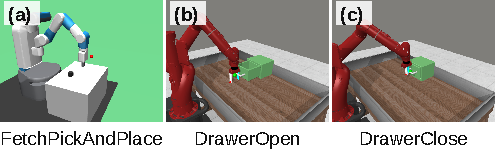
\includegraphics[width=\columnwidth]{figures/experimental_task_panels.pdf}
\caption{Illustrative simulator renderings of the experimental tasks. The panels are not evaluation rollouts.}
\label{fig:experimental-environments}
\end{figure}

\paragraph{Evaluation and statistics.}
Policies are evaluated deterministically over 20 episodes at each checkpoint. Paired analyses use only exact shared evaluation steps, without smoothing, interpolation, or filling. Normalized success AUC over the complete shared evaluation span is the primary metric because it captures both learning speed and sustained performance under a fixed interaction budget. Final-quarter success AUC is a secondary late-training summary: it applies the same normalized trapezoidal calculation to the final 25\% of the environment-step budget, namely 750k--1M on FPP and 1.5M--2M on the Drawer tasks. Final success is also secondary; Hit90 (the first checkpoint with success \(\geq 0.9\), with reached-seed coverage) is reported in the supplement. We report seed means and sample standard deviations; paired claims use within-seed differences and 10,000-resample percentile-bootstrap 95\% confidence intervals. Absolute AUC values are not compared across tasks with different horizons or budgets.

\subsection{Primary Comparisons}

\paragraph{Comparison setup.}
HER addresses sparse supervision through goal relabeling, but learning effort can be reallocated at several stages of the training pipeline. HGR prioritizes episodes and transition--future-goal pairs by TD error with two-stage importance correction~\citep{luu2021hgr}, whereas PER samples replay transitions by TD-error priority with annealed importance correction~\citep{schaul2016per}. SABER preserves both selections and changes only the critic-loss coefficients within the sampled and relabeled minibatch. These methods therefore intervene at distinct points in the HER actor--critic pipeline.

Additional validated DDPG and SAC controls comparing support-based and TD-error-based critic-loss weighting under uniform replay are reported in the supplement. AER~\citep{sun2020aer}, high-replay-ratio HER, and REDQ-HER variants~\citep{chen2021redq,hiraoka2023sparsegoalredq} are retained there as secondary scaling references because they also change HER usage, update budget, or architecture.

% Overleaf-ready compact table snippet.
% Requires: \usepackage{booktabs}
\begin{table*}[t]
\centering
\caption{Primary post-HER comparisons over paired seeds 1--5.
Entries are mean $\pm$ sample standard deviation; Hit90 is the median
first step reaching $90\%$ success, with reached-seed coverage in parentheses.
Repeated \emph{HER+} prefixes are omitted for compactness.
SABER denotes our method, and its reported values are shown in bold.
FPP SAC uses the exact common 50k--1M evaluation grid.}
\label{tab:primary-posther-comparisons}

\setlength{\tabcolsep}{1.2pt}
\renewcommand{\arraystretch}{1.02}
\fontsize{7}{7.8}\selectfont
\setlength{\heavyrulewidth}{0.8pt}
\setlength{\lightrulewidth}{0.4pt}

\begin{minipage}[t]{0.326\textwidth}
\vspace{0pt}
\centering
\textit{\strut FetchPickAndPlace (FPP; 1M)}
\par\vspace{2pt}
\begin{tabular*}{\linewidth}{@{\extracolsep{\fill}}lccc@{}}
\toprule
Method & Final & AUC & Hit90 \\
\midrule
\multicolumn{4}{@{}l}{DDPG} \\
\textbf{SABER}
  & \(\mathbf{0.960 \pm .042}\) & \(\mathbf{0.609 \pm .038}\)
  & \textbf{540k (5/5)} \\
HER
  & \(0.940 \pm .042\) & \(0.539 \pm .125\) & 600k (5/5) \\
HGR
  & \(0.540 \pm .365\) & \(0.338 \pm .149\) & 930k (2/5) \\
\shortstack[l]{TD-error\\weighting}
  & \raisebox{3.5pt}{\(0.930 \pm .104\)}
  & \raisebox{3.5pt}{\(0.568 \pm .069\)}
  & \raisebox{3.5pt}{630k (5/5)} \\
Full PER
  & \(0.780 \pm .438\) & \(0.460 \pm .238\) & 640k (4/5) \\
\addlinespace[1pt]
\multicolumn{4}{@{}l}{TD3} \\
\textbf{SABER}
  & \(\mathbf{0.970 \pm .045}\) & \(\mathbf{0.442 \pm .035}\)
  & \textbf{840k (5/5)} \\
HER
  & \(0.840 \pm .188\) & \(0.372 \pm .032\) & 980k (3/5) \\
HGR
  & \(0.610 \pm .198\) & \(0.367 \pm .034\) & 630k (1/5) \\
\shortstack[l]{TD-error\\weighting}
  & \raisebox{3.5pt}{\(0.490 \pm .171\)}
  & \raisebox{3.5pt}{\(0.351 \pm .021\)}
  & \raisebox{3.5pt}{630k (1/5)} \\
Full PER
  & \(0.660 \pm .204\) & \(0.369 \pm .034\) & 1.00M (1/5) \\
\addlinespace[1pt]
\multicolumn{4}{@{}l}{SAC} \\
\textbf{SABER}
  & \(\mathbf{0.990 \pm .022}\) & \(\mathbf{0.583 \pm .030}\)
  & \textbf{750k (5/5)} \\
HER
  & \(0.790 \pm .288\) & \(0.471 \pm .079\) & 800k (3/5) \\
HGR
  & \(0.760 \pm .251\) & \(0.484 \pm .071\) & 800k (2/5) \\
\shortstack[l]{TD-error\\weighting}
  & \raisebox{3.5pt}{\(0.990 \pm .022\)}
  & \raisebox{3.5pt}{\(0.544 \pm .068\)}
  & \raisebox{3.5pt}{800k (5/5)} \\
Full PER
  & \(0.990 \pm .022\) & \(0.690 \pm .046\) & 550k (5/5) \\
\bottomrule
\end{tabular*}
\end{minipage}
\hfill
\begin{minipage}[t]{0.326\textwidth}
\vspace{0pt}
\centering
\textit{\strut DrawerOpen (2M)}
\par\vspace{2pt}
\begin{tabular*}{\linewidth}{@{\extracolsep{\fill}}lccc@{}}
\toprule
Method & Final & AUC & Hit90 \\
\midrule
\addlinespace[19.8373pt]
\multicolumn{4}{@{}l}{DDPG} \\
\textbf{SABER}
  & \(\mathbf{1.000 \pm .000}\) & \(\mathbf{0.754 \pm .044}\)
  & \textbf{500k (5/5)} \\
HER
  & \(0.390 \pm .534\) & \(0.207 \pm .287\) & 960k (2/5) \\
HGR
  & \(0.900 \pm .224\) & \(0.688 \pm .142\) & 530k (5/5) \\
\shortstack[l]{TD-error\\weighting}
  & \raisebox{3.5pt}{\(0.800 \pm .447\)}
  & \raisebox{3.5pt}{\(0.715 \pm .090\)}
  & \raisebox{3.5pt}{610k (5/5)} \\
Full PER
  & \(0.990 \pm .022\) & \(0.825 \pm .044\) & 330k (5/5) \\
\addlinespace[19.8373pt]
\multicolumn{4}{@{}l}{TD3} \\
\textbf{SABER}
  & \(\mathbf{0.590 \pm .539}\) & \(\mathbf{0.362 \pm .338}\)
  & \textbf{780k (3/5)} \\
HER
  & \(0.190 \pm .425\) & \(0.127 \pm .283\) & 740k (1/5) \\
HGR
  & \(0.580 \pm .531\) & \(0.371 \pm .343\) & 760k (3/5) \\
\shortstack[l]{TD-error\\weighting}
  & \raisebox{3.5pt}{\(0.400 \pm .548\)}
  & \raisebox{3.5pt}{\(0.202 \pm .284\)}
  & \raisebox{3.5pt}{1.015M (2/5)} \\
Full PER
  & \(0.600 \pm .548\) & \(0.406 \pm .374\) & 720k (3/5) \\
\addlinespace[19.8373pt]
\bottomrule
\end{tabular*}
\end{minipage}
\hfill
\begin{minipage}[t]{0.326\textwidth}
\vspace{0pt}
\centering
\textit{\strut DrawerClose (2M)}
\par\vspace{2pt}
\begin{tabular*}{\linewidth}{@{\extracolsep{\fill}}lccc@{}}
\toprule
Method & Final & AUC & Hit90 \\
\midrule
\addlinespace[19.8373pt]
\multicolumn{4}{@{}l}{DDPG} \\
\textbf{SABER}
  & \(\mathbf{0.280 \pm .251}\) & \(\mathbf{0.324 \pm .082}\)
  & \textbf{20k (5/5)} \\
HER
  & \(0.160 \pm .182\) & \(0.251 \pm .030\) & 70k (5/5) \\
HGR
  & \(0.080 \pm .091\) & \(0.349 \pm .184\) & 100k (5/5) \\
\shortstack[l]{TD-error\\weighting}
  & \raisebox{3.5pt}{\(0.400 \pm .166\)}
  & \raisebox{3.5pt}{\(0.313 \pm .098\)}
  & \raisebox{3.5pt}{130k (5/5)} \\
Full PER
  & \(0.460 \pm .363\) & \(0.308 \pm .049\) & 60k (5/5) \\
\addlinespace[19.8373pt]
\multicolumn{4}{@{}l}{TD3} \\
\textbf{SABER}
  & \(\mathbf{0.590 \pm .539}\) & \(\mathbf{0.549 \pm .422}\)
  & \textbf{80k (5/5)} \\
HER
  & \(0.350 \pm .480\) & \(0.329 \pm .348\) & 70k (5/5) \\
HGR
  & \(0.500 \pm .457\) & \(0.602 \pm .305\) & 80k (5/5) \\
\shortstack[l]{TD-error\\weighting}
  & \raisebox{3.5pt}{\(0.200 \pm .447\)}
  & \raisebox{3.5pt}{\(0.369 \pm .275\)}
  & \raisebox{3.5pt}{30k (5/5)} \\
Full PER
  & \multicolumn{3}{c}{\textit{pending}} \\
\addlinespace[19.8373pt]
\bottomrule
\end{tabular*}
\end{minipage}
\end{table*}


Table~\ref{tab:primary-posther-comparisons} summarizes final success, full-span success AUC, and final-quarter success AUC across all task--backbone cohorts. Hit90 and reached-seed coverage are reported in the supplement as complementary measures of learning speed and reliability. Figure~\ref{fig:primary-fpp-backbone-curves} shows FPP learning dynamics across all three backbones.

\begin{figure*}[t]
\centering
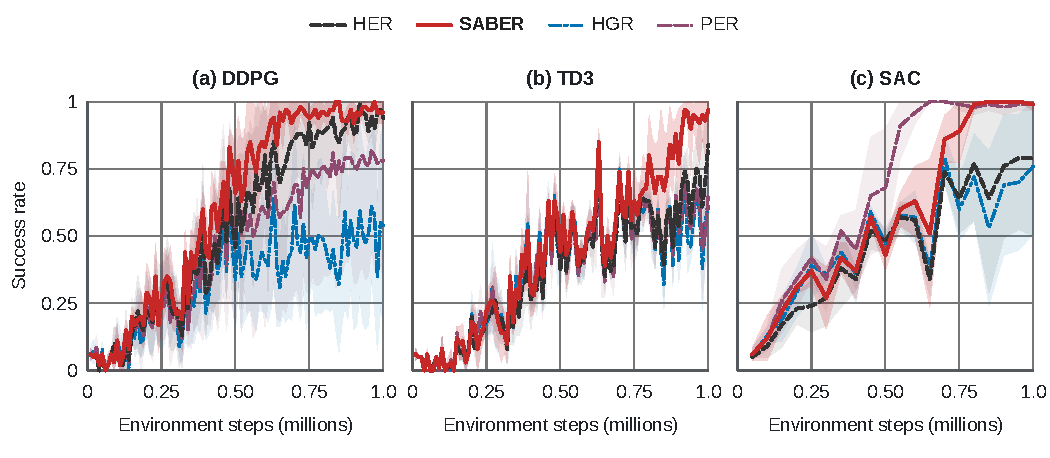
\includegraphics[width=0.85\textwidth]{figures/primary_fpp_backbone_learning_curves.pdf}
\caption{FetchPickAndPlace learning curves for the primary comparisons across
DDPG, TD3, and SAC. Lines show mean deterministic evaluation success over
paired seeds 1--5, and shaded regions show sample standard deviation. DDPG
and TD3 use the exact 10k evaluation grid, while SAC uses the exact shared
50k grid. No smoothing or interpolation is applied; corresponding full-span
AUC, final-quarter AUC, and final-success values are reported in
Table~\ref{tab:primary-posther-comparisons}.}
\label{fig:primary-fpp-backbone-curves}
\end{figure*}

\paragraph{Matched HER comparison.}
SABER achieves higher mean full-span AUC than matched HER in all seven cohorts, with paired 95\% confidence intervals excluding zero in four (Table~\ref{tab:primary-posther-comparisons}). A frozen FPP TD3 extension to ten paired seeds yields a mean difference of \(+0.0467\) (95\% CI \([0.0085,0.0783]\)), with SABER higher in 8/10 pairs. Under the inclusive future-goal convention, the five-seed mean gain is \(+0.0674\) (95\% CI \([-0.0068,0.1416]\)), compared with \(+0.0708\) under the primary convention; the observed mean direction is the same, but this is not an equivalence test. DrawerOpen DDPG shows the largest gain, from \(0.207\) to \(0.754\), and final-quarter AUC favors SABER in all seven cohorts. Seed-level confirmatory and sensitivity results are reported in the supplement.

\paragraph{HGR comparison.}
HGR and SABER address different allocation decisions in HER-based learning: HGR changes which hindsight experiences enter an update, whereas SABER changes the relative critic-fitting contribution of experiences already selected. SABER achieves higher mean full-span AUC on all three FPP backbones and on DrawerOpen DDPG. HGR is slightly higher on DrawerOpen TD3 and higher on both DrawerClose backbones. On DrawerClose, however, SABER has higher observed final-quarter AUC: \(0.277\) versus \(0.226\) with DDPG and \(0.534\) versus \(0.460\) with TD3. The paired intervals for these late-training differences include zero, so the result indicates a metric-dependent, task-dependent ordering rather than stronger evidence of stability or a universal ranking. In our recorded implementations, HGR has lower throughput than SABER in every evaluated cohort; these hardware-specific measurements are reported separately and are not used as a performance claim.

\paragraph{PER comparison.}
Across all seven cohorts, PER produces a mixed ordering. SABER has higher mean full-span AUC on FPP DDPG, FPP TD3, and both DrawerClose backbones, whereas PER is higher on FPP SAC and both DrawerOpen backbones. DrawerClose TD3 also exposes a metric trade-off: SABER attains higher full-span AUC (\(0.549\) versus \(0.524\)), whereas PER has higher final-quarter AUC (\(0.583\) versus \(0.534\)) and marginally higher mean final success (\(0.600\) versus \(0.590\)). PER changes the replay distribution and applies importance correction, so it is a broader replay-selection intervention rather than a matched loss-allocation control. Neither replay prioritization nor critic-loss allocation therefore uniformly dominates across tasks, backbones, and metrics.

\subsection{Diagnostic Instrumentation}

Diagnostic logging adds no gradient terms and does not alter replay sampling, training objectives, or the parameter-update order. For FPP, we record one full minibatch every 10k environment steps for seeds 1--5 of DDPG, TD3, and SAC, yielding 500 diagnostic batches per backbone and 1,500 in total. DrawerOpen and DrawerClose DDPG use primary five-seed diagnostic cohorts. Snapshot-level quantities are first averaged within each seed, and seeds are treated as the independent analysis units.

\paragraph{Support activation.}
We first measure how often SABER's support condition activates during training. The support-positive rate is the fraction of logged samples for which \(\psi_i=1\). Across the five instrumented cohorts, it ranges from \(0.197\) on FPP SAC to \(0.429\) on DrawerOpen DDPG. Thus, the indicator consistently identifies a nontrivial subset of each minibatch rather than degenerating to an almost-always or almost-never signal. Complete cohort-level estimates are reported in the supplement.

\paragraph{TD-error enrichment.}
We next relate support to the pre-update absolute Bellman residual \(|\delta_i^{\mathrm{pre}}|\). On FPP, Pearson correlations with the binary indicator are weak (\(0.116\)--\(0.143\)), whereas support-positive rates in the top TD-error decile are enriched by \(1.409\times\)--\(1.828\times\) over their base rates. DrawerOpen and DrawerClose show support-positive/negative residual ratios of \(1.17\times\) and \(1.42\times\), respectively, with the same direction in all five seeds of each cohort. Support-positive samples are therefore enriched among high-error samples without reducing to a TD-error ranking.

\paragraph{One-update residual reduction.}
To test whether support-conditioned weights affect the intended critic update, we hold the Bellman targets fixed and measure \(|\delta_i^{\mathrm{pre}}|-|\delta_i^{\mathrm{post}}|\) on the same minibatch after one critic step. Support-positive/negative reduction ratios are \(2.39\times\), \(3.30\times\), and \(3.94\times\) for FPP DDPG, TD3, and SAC, and \(2.10\times\) and \(2.94\times\) for DrawerOpen and DrawerClose. The positive-sample reduction is larger in all 25 backbone--seed runs. These results verify that SABER translates its support signal into the intended redistribution of immediate critic fitting; the independent contribution of exact sample assignment is evaluated in the subsequent ablations.


\paragraph{Phase-conditioned allocation.}
Finally, we examine where support activates along Drawer task progression using phases conditioned on the relabeled training goal. The completed open and closed phases account for \(73.8\%\) and \(74.7\%\) of logged samples, respectively, but have the lowest support-positive rates (\(0.326\) and \(0.212\)). SABER therefore activates more frequently around approach and drawer interaction than in the dominant terminal phase. Full phase definitions, counts, and seed-level results are reported in the supplement.

\subsection{Mechanism Ablations}

The primary comparisons establish SABER's performance gains but not whether they arise from the support query, its pairing with the sampled context, or the placement of high critic weights. We evaluate four DDPG controls on FPP, DrawerOpen, and DrawerClose with paired seeds 1--5, while retaining SABER's training budget, HER and replay procedures, support hyperparameters, critic-only scope, UTD ratio, and evaluation protocol. Table~\ref{tab:mechanism-ablations} reports paired SABER-minus-control AUC differences; positive values favor SABER.

\paragraph{Replay-Action Query.}
Replay-Action Query replaces \(a_i^\pi\) with \(a_i^r\) only in the support query, retaining the context, population threshold, weight computation, replay-action regression, and actor objective. Because the sampled transition remains in its local replay pool, its replay action can support itself within the bounded scan. SABER is higher on all three tasks, with the interval excluding zero only on DrawerOpen (Table~\ref{tab:mechanism-ablations}), showing that query identity can materially affect learning.

\paragraph{Shuffled-Policy Query.}
Shuffled-Policy Query applies a fixed-point-free within-minibatch permutation to the current-policy actions, preserving their multiset while breaking sample--query pairing. The shuffled action is used only for the support query, and its weight remains attached to the original replay-action residual. SABER is higher on all three tasks, although all intervals include zero. Because Replay-Action and Shuffled-Policy Query can also change the support-positive count, they test the overall effects of query identity and pairing rather than alignment under a matched count.

\paragraph{Random-Support.}
At each update, Random-Support applies SABER's indicator rule to the control run's own minibatch and replay state, obtains a counterfactual mask $M$ with $k=\sum_i M_i$, and assigns exactly $k$ high weights uniformly without replacement across the minibatch. It matches the support-positive count induced by the SABER rule, as well as the raw and normalized weight distributions, while removing sample-level context eligibility and action-bin membership from the high-weight locations. SABER is higher on all three tasks, with the FPP interval excluding zero. Because $k$ is still determined by SABER's support rule, this is a count-matched control rather than a support-free baseline.

\paragraph{Context-Eligible Count-Matched.}
This stricter control draws the same $k$ samples without replacement only from the eligible set $E$ defined by SABER's local-context population threshold. It therefore also matches context eligibility, leaving current-policy action-bin membership as the only intended algorithmic difference. SABER is higher on all three tasks, but all intervals include zero. The direction is consistent with membership-aligned assignment contributing, but does not independently establish exact support membership as the unique causal mechanism.

\begin{table}[!t]
\centering
\small
\setlength{\tabcolsep}{1.25pt}
\newcommand{\mechanismrowsep}{%
  \noalign{\vskip6.5pt%
    \hbox to \dimexpr\columnwidth-2pt\relax{%
      \leaders\hbox to 4pt{\hfil\raisebox{0.35ex}[0pt][0pt]{\rule{0.5pt}{0.5pt}}\hfil}\hfill}%
    \vskip6.5pt}}
\begin{tabular}{@{}lccc@{}}
\toprule
Control & FPP & Open & Close \\
\specialrule{\lightrulewidth}{\aboverulesep}{6.5pt}
\shortstack[l]{Replay-Action\\Query}
  & \shortstack{\(+0.011\)\\\([-0.028,0.059]\)}
  & \shortstack{\(+0.436\)\\\([0.121,0.729]\)}
  & \shortstack{\(+0.049\)\\\([-0.006,0.128]\)} \\
\mechanismrowsep
\shortstack[l]{Shuffled-Policy\\Query}
  & \shortstack{\(+0.043\)\\\([-0.002,0.085]\)}
  & \shortstack{\(+0.105\)\\\([-0.080,0.335]\)}
  & \shortstack{\(+0.033\)\\\([-0.063,0.119]\)} \\
\mechanismrowsep
\shortstack[l]{Random-\\Support}
  & \shortstack{\(+0.056\)\\\([0.014,0.101]\)}
  & \shortstack{\(+0.047\)\\\([-0.042,0.136]\)}
  & \shortstack{\(+0.048\)\\\([-0.004,0.115]\)} \\
\mechanismrowsep
\shortstack[l]{Context-Eligible\\Count-Matched}
  & \shortstack{\(+0.033\)\\\([-0.006,0.076]\)}
  & \shortstack{\(+0.149\)\\\([-0.042,0.442]\)}
  & \shortstack{\(+0.030\)\\\([-0.033,0.092]\)} \\
\specialrule{\heavyrulewidth}{6.5pt}{0pt}
\end{tabular}
\caption{Paired SABER-minus-control normalized success AUC differences
(95\% paired-bootstrap CIs), using DDPG seeds 1--5.
Open and Close denote DrawerOpen and DrawerClose;
positive values favor SABER.}
\label{tab:mechanism-ablations}
\end{table}

\subsection{Current Scope and Future Work}

Our evaluation is limited to three simulated manipulation tasks and five-seed primary cohorts, with no matched SAC results on the Drawer tasks. SABER also depends on task-specific discretized contexts, fixed support thresholds, and bounded replay retrieval, while incurring support-query overhead not captured by the matched UTD ratio. It does not address exploration when useful current-policy actions are absent from replay. Future work should examine adaptive support representations, more efficient retrieval, broader tasks, and larger-scale evaluation.

\section{Conclusion}

We introduced SABER, a critic-only post-HER objective that reallocates Bellman-loss coefficients according to local replay support for current-policy actions while leaving replay sampling, HER relabeling, Bellman targets, actor objectives, architectures, and UTD unchanged. SABER achieved higher mean normalized success AUC than matched HER across all seven task--backbone cohorts, and diagnostics confirmed that its support signal produces the intended redistribution of critic fitting. HGR and PER remained stronger in some settings, indicating that critic-loss reweighting complements rather than universally replaces replay prioritization. These results show that HER-based learning can improve by changing how critic supervision is distributed, even when the sampled and relabeled experience itself remains unchanged.

\bibliography{saber_refs}

\end{document}
